\documentclass[11pt]{article}

\usepackage[T1]{fontenc}
\usepackage{geometry}
\usepackage{amsmath, amssymb, amsthm}
\usepackage{listings}
\usepackage{xcolor}
\usepackage{graphicx}
\usepackage{caption}
\usepackage{float}
\usepackage{siunitx}

\geometry{a4paper, margin=1in, headheight=14pt}

\definecolor{darkgreen}{rgb}{0.2, 0.6, 0.4}
\definecolor{darkblue}{rgb}{0.2, 0.4, 0.8}
\lstset{ 
  basicstyle=\footnotesize\ttfamily,
  commentstyle=\color{gray},
  % extendedchars=true,
  % keepspaces=true,
  keywordstyle=\color{darkblue},
  % numbers=left,
  % numbersep=5pt,
  % numberstyle=\tiny\color{gray},
  stringstyle=\color{darkgreen},
  tabsize=4,
  % frame=lines,
  aboveskip=2em,
  belowskip=2em
}

\newcommand\dd[2]{\frac{d #1}{d #2}}
\newcommand\pp[2]{\frac{\partial #1}{\partial #2}}

\title{
    \Large\textsc{PH2203: Physics Laboratory IV} \\
    \vspace{5pt}
    \LARGE{Calculation of gravitational acceleration using a pendulum and the
    Doppler effect}
}
\author{
    \large Satvik Saha%
    \thanks{Email: \tt ss19ms154@iiserkol.ac.in}
    \\\textsc{\small 19MS154}
}
\date{\normalsize
    \textit{Indian Institute of Science Education and Research, Kolkata, \\
    Mohanpur, West Bengal, 741246, India.} \\
    \vspace{10pt}
    \today
}

\begin{document}
    \maketitle

    \begin{abstract}
        In this experiment, we use two principles to measure the local gravitational
        acceleration, namely the relationship between the frequency of oscillation of a
        simple pendulum with its length $\ell$ and gravitational acceleration $g$,
        as well as the Doppler effect.
    \end{abstract}

    \section{Experimental setup}
    The pendulum consists of a platform suspended by four strings of equal length
    $\ell$ by its corners. A smartphone, which acts as an acoustic sensor, is placed
    on it, and the pendulum is allowed to oscillate with a small angular
    displacement. A stationary source of sound of frequency $\nu_0 = \SI{1000}{\Hz}$ is
    placed such that the smartphone moves precisely towards and away from the source
    as it oscillates. The frequency $\nu$ measured by the smartphone thus varies
    in time with the oscillations, which is used to measure the frequency of
    oscillation. This in turn is used to calculate $g$.
    
    \begin{figure}[H]
    \begin{center}
        \includegraphics[scale=1.0]{./pendulum.eps}
    \end{center}
    \caption{A schematic of the experimental setup.}
    \label{fig:setup}
    \end{figure}

    \section{Theory}
    The motion of the pendulum can be approximated to be equivalent to that of a
    simple pendulum. Note that the platform does not rotate in space, and hence
    contributes no angular momentum. The Lagrangian is thus \[
        \mathcal{L} = T - V = \frac{1}{2}m\ell^2\dot{\theta}^2 + mg\ell\cos\theta,
    \] which is identical to that of a simple pendulum. Solving the Euler-Lagrange
    equation \[
        \dd{}{t}\left(\pp{\mathcal{L}}{\dot{\theta}}\right) =
        \pp{\mathcal{L}}{\theta},
    \] and using $\sin\theta \approx \theta$ for small oscillations, we recover \[
        \ddot{\theta} + \frac{g}{\ell}\theta = 0,
    \] whence \[
        \theta(t) = \theta_0 \cos(\omega t),
    \] $\omega^2 = g / l$. The time period of oscillation is given by \[
        T = \frac{2\pi}{\omega} = 2\pi \sqrt{\frac{\ell}{g}}.
    \] Rearranging for $g$, and setting the frequency of oscillation $f = 1 / T$, \[
        g = 4\pi^2 \ell f^2. \tag{\star}
    \] 
    Note that \[
        \dot{\theta}(t) = -\omega\theta_0\sin(\omega t),
    \] so the velocity $v \approx \ell\dot{\theta}$ of the pendulum in the direction
    of our sound source also oscillates with frequency $f$. Since the frequency of
    sound detected by our smartphone varies as \[
        \nu = \nu_0\left(1 + \frac{v}{v_0}\right),
    \] the frequency $\nu$ also oscillates with frequency $f$. This means that we
    can extract $f$ from the detected waveform, either by counting the number of
    oscillations over some time or by performing a Fourier transform. This along
    with $\ell$ will give a value for $g$.


    \section{Measurements}
    The effective length of the pendulum has been approximated as the length of the
    strings, recorded using a tape measure and averaged.
    The frequency of oscillation has been calculated by observing 30 oscillations in
    $\nu$ over a period of \SI{40}{\s}, and has been confirmed by performing a
    Fourier transform on the data.

    We report \[
        \ell \approx \SI{44}{\cm}, \qquad
        f \approx \SI{0.75}{\Hz}.
    \] 
    
    \begin{figure}[H]
    \begin{center}
        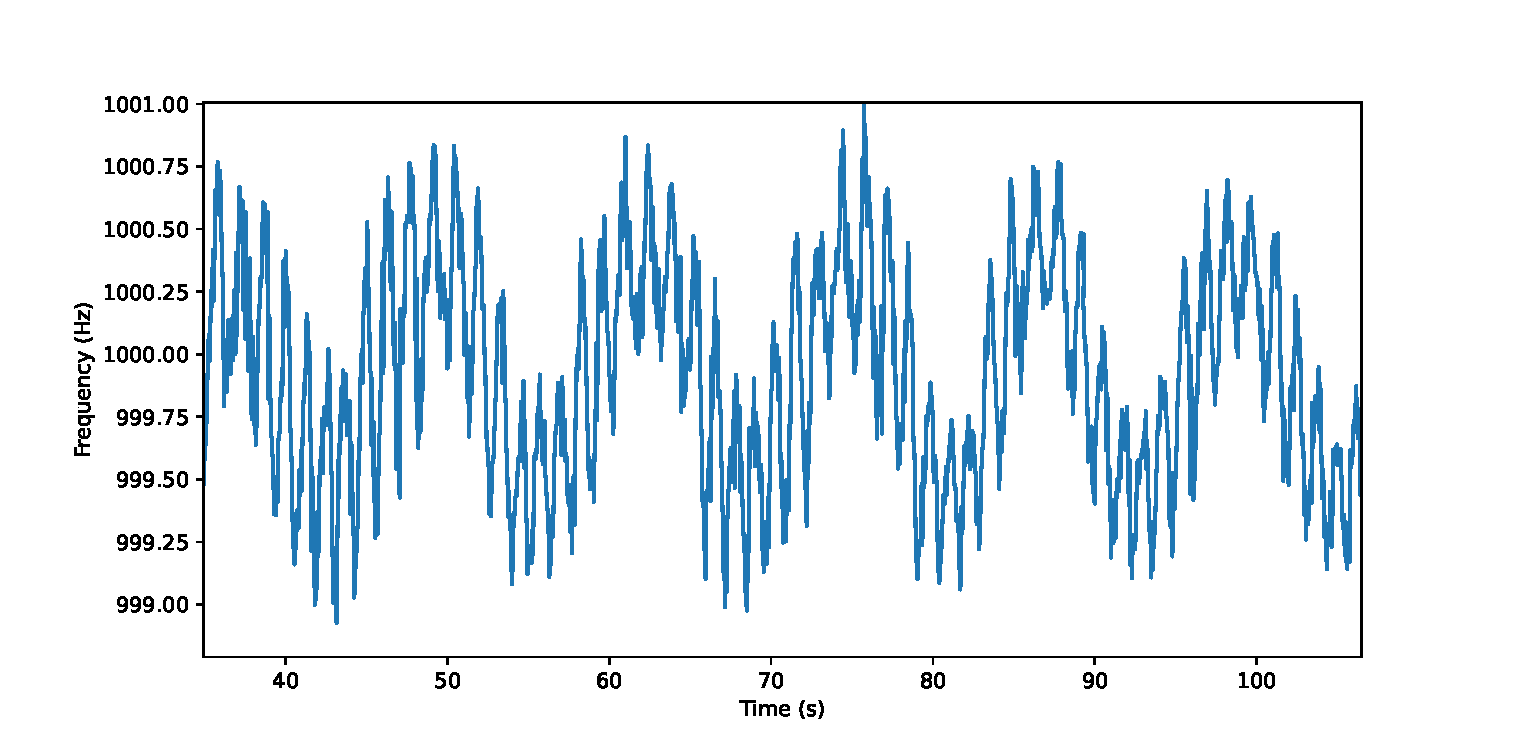
\includegraphics[width=\textwidth]{./freq.eps}
    \end{center}
    \caption{A sample of the data collected, zoomed in for clarity.}
    \label{fig:freq}
    \end{figure}
    
    \begin{figure}[H]
    \begin{center}
        \includegraphics[width=0.7\textwidth]{./fourier.eps}
    \end{center}
    \caption{The Fourier transform of the frequency data, around $f =
    \SI{0.75}{\Hz}$.}
    \label{fig:fourier}
    \end{figure}

    \section{Calculations}
    Using our working formula (\star), \[
        g = 4\pi^2\ell f \approx 4\pi^2\cdot \SI{0.44}{\m}\cdot
        \left(\SI{0.75}{\per\s}\right)^2 \approx \SI{9.77}{\m\per\s^2}.
    \] 

    \section{Error analysis}
    To get an upper estimate on the error in $g$, we differentiate (\star) and write
    \[
    \frac{\delta g}{g} \approx \frac{\delta\ell}{\ell} + 2\,\frac{\delta f}{f}.
    \] We estimate $\delta\ell = \SI{0.5}{\cm}$ and $\delta f = 0.005$.
    Thus, we claim a relative error of \[
        \frac{\delta g}{g} \approx 0.025 = \SI{2.5}{\percent},
    \] with a reported value of \[
        g \,=\, {9.77 \pm 0.24}\;\si{\m\per\s^2}.
    \] Given that the standard value of gravitational acceleration is around
    \SI{9.79}{\m\per\s^2}, we have an absolute error of \SI{-0.02}{\m\per\s^2}, with
    a percentage error of \SI{-0.2}{\percent}. This of course ignores factors such
    as elevation and local features, whose effect may be considered negligible.
    
    \section{Discussion}
    We have measured the local acceleration due to gravity with some accuracy.

    The frequency curve in Figure.~\ref{fig:freq} displays oscillations apart from
    the one caused by the Doppler effect, specifically the large sinusoidal
    oscillation with a time period of around \SI{15}{\s}. This persists even when
    the smartphone is placed on a stationary surface, and is likely an artefact of
    the speaker-microphone combination.
    
    
\end{document}
% vim: set tabstop=4 shiftwidth=4 softtabstop=4:
